
Modeling a system's vulnerabilities and the reachability between those vulnerabilities can be found in the literature as far back as 1994 with Dacier\cite{Dacier_1994} formalising the concept of privilege graphs and representing the translated graph as a Markov Model. Phillips and Swiler\cite{Phillips_Swiler_1998} present a separate attack graph generation method that can account for multi-stage attacks and attacker capabilities in 1998. In 1999 Ortalo\cite{Ortalo_1999}  provides experimental results and some fundamental metrics using Markov analysis with Dacier's privilege graphs, and in 2002 Sheyner\cite{Sheyner_Haines_Jha_Lippmann_Wing_2002} describes how attack graph construction and analysis can be automated. In 2006 Ou\cite{Ou_Boyer_McQueen_2006} provides an analysis of scalability extensions to the MulVal\cite{Ou_Govindavajhala_Appel} attack graph engine presented the previous year, and in 2013 Hong\cite{Hong_Kim_Takaoka_2013} presents further scalability improvements to MulVal using logic reduction techniques. In 2015 Abraham\cite{Abraham_Nair_2015b} introduces the Cyber Security Analytics Framework(CSAF) which we adopt for this analysis. More thorough surveys of the canonical attack graph literature can be found in \cite{Kordy_2013} and \cite{Lippmann_Ingols_2005}. We use the remainder of this section to illustrate the MulVal inputs and outputs as expected by the CSAF. 

Attack graphs show the relationships among vulnerabilities within a system and provide context to security scans already conducted by many organisations. An attack graph is a directed graph that captures all possible paths an attacker can traverse within a system to reach a desired target state. The first node in the graph represents the origin of the attack and the final node denotes the target. The origin contains only outbound edges and the target contains only inbound edges. Nodes in the graph between the origin and target represent discrete states in states network. Each edge in the graph identifies a possible pivot from one state to another through either unaltered access mechanisms or successful exploitation of a vulnerability. The conditions necessary for successful compromise of the vulnerability are encapsulated in the attack graph vertices, and include information such as network, port, protocol, and access privilege level restrictions, as well as the effect of a successful exploit on the system such as privilege escalation or remote code execution. These conditions can be populated from the output of IA and network management systems, or in hypothetical cases, can be defined manually.  

%Our research extends the insight provided by an attack graph to draw conclusions about the security of a network through analyzing these vulnerability relationships and simulating an attacker’s progression through the network to a given target.   

% \begin{figure}[H]
% \centering
% \begin{adjustbox}{minipage=\linewidth,scale=0.6}
% \begin{subfigure}{.5\textwidth}
% \includegraphics[width=\linewidth]{img/eg_net.png}
% \caption{example network}
% \label{fig:eg_net}
% \end{subfigure}%
% \begin{subfigure}{.5\textwidth}
% %%\includegraphics[width=\linewidth]{img/1553187466080.png}
% 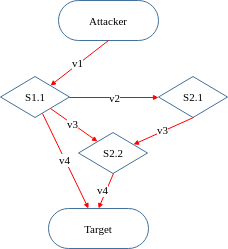
\includegraphics[width=\linewidth]{content/figs/eg_attack_graph_002a.png}
% \caption{resulting attack graph}
% \label{fig:eg_ag}
% \end{subfigure}%
% \caption{Attack Graph Example}
% \label{fig:eg}
% \end{adjustbox}
% \end{figure} 

% For example, Figure \ref{fig:eg_net} shows a fictional system being targeted by an attacker and Figure \ref{fig:eg_ag} shows the derived attack graph. While there exist 4 vulnerabilities between the attacker and the target, only vulnerability v1 is exploitable from the attacker’s original context. If this vulnerability is successfully exploited, the attacker can subsequently exploit vulnerabilities v2 or v3 on System 2 or proceed directly to the Target by exploiting v4. Note in Figure \ref{fig:eg_ag} that nodes S2.1 and S2.2 are separate vulnerabilities on the same system (System 2); nodes in an attack graph don’t necessarily have a one-to-one mapping to system elements. Also notice that there are three possible attack paths available for the attacker to reach the target.  


% The next step is to take the generated attack graph and augment transition probabilities based on an established or approximated CVSS score.  For example, we may choose exploitability, the measure of how easily a vulnerability is leveraged by an attacker, or impact, the measure of how critical an exploit would be to operations, to base the likelihood of an attack path being taken. Due to the large and complex graphs that can be generated for even simple networks, we automate the process of translating the attack graph output into a form that can be consumed by subsequent phases through a data transform pipeline to include graph node reduction, CVSS score lookup and assignment, and transition probability calculations.

The example in Figure \ref{fig:eg_net01} assumes an attacker located on the public internet with the target being root access on the internal workstation. The network model provided to MulVal is shown in Listing \ref{lst:input}. The $hacl/4$ clauses define access control rules that depict router and firewall configurations and dictate reachability between states. The host configuration properties include what services are running, the user or privilege level that service is running as, and any vulnerabilities known to affect that service.



% % \begin{minipage}{.45\textwidth}
% \begin{lstlisting}[style=datalog, label={lst:input}, caption={input.P \cite{Ou_Boyer_McQueen_2006}},  linewidth=.48\textwidth, xleftmargin=20pt]]
% attackerLocated(internet).
% attackGoal(execCode(workStation,_)).
% hacl(internet, webServer, tcp, 80).
% hacl(webServer, _,  _, _).
% hacl(fileServer, _, _, _).
% hacl(workStation, _, _, _).
% hacl(H,H,_,_).
% /* configuration information of fileServer */
% networkServiceInfo(fileServer, mountd, rpc, 100005, root).
% nfsExportInfo(fileServer, '/export', _anyAccess, workStation).
% nfsExportInfo(fileServer, '/export', _anyAccess, webServer).
% vulExists(fileServer, vulID, mountd).
% vulProperty(vulID, remoteExploit, privEscalation).
% localFileProtection(fileServer, root, _, _).
% /* configuration information of webServer */
% vulExists(webServer, 'CAN-2002-0392', httpd).
% vulProperty('CAN-2002-0392', remoteExploit, privEscalation).
% networkServiceInfo(webServer , httpd, tcp , 80 , apache).
% /* configuration information of workStation */
% nfsMounted(workStation, '/usr/local/share', 
%   fileServer, '/export', read).
% \end{lstlisting}
% % \end{adjustbox}
% % \end{minipage}
% % \end{tabular}
% % \end{figure*}

% \begin{lstlisting}[style=datalog, label={lst:input}, caption={current.P},  linewidth=.48\textwidth, xleftmargin=20pt]]


% /*
% Current Network State Model
% */


% /*
%   attacker is at the customer edge or internet 
%   pe1 is CRS with vuln CVE-2012-1342 (ACL bypass)
%   target is core router p3 control plane code execution

% _c control plane interface
% _d data plane interface
% _m management interface
% */
% attackerLocated(ce1).
% attackGoal(execCode(p3_c, _)).

% /*
% Customer Edge devices attach to Provider Edges
% control plane to exchange routing tables/VRFs
% through BGP
% */
% /* BGP b/t customer and provider edge */
% /* update 20160425: data and control from customer on same PE port */
% /*hacl(ce1, pe1_c,  tcp, 179).*/
% hacl(ce1, pe1_d,  _, _). 

% /* Customer data flows pass through PE data plane
% on any port/protocol '_'
% */
% /* update 20160425: data and control from customer on same PE port */
% hacl(pe1_d, pe1_c,  _, _).
% /*
% hacl(ce1, pe1_c,  _, _).
% hacl(pe1_d, pe1_c,  _, _).
% hacl(pe1_c, pe1_d,  _, _).   
% */

% /* ???
% Provider Edge devices pass data through other PE's?
% */
% /*Customer data flows pass through PE data plane
% on any port/protocol '_' */
% hacl(pe1_d, pe2_d, _ , _).
% hacl(pe1_d, pe4_d, _ , _).
% hacl(pe2_d, pe3_d, _ , _).
% hacl(pe3_d, pe4_d, _ , _).

% /*
% Provider Edge devices talk to other PEs
% BGP b/t provider edges control plane
% exchange client VRFs 
% */
% hacl(pe1_c, pe2_c,  TCP, 179).
% hacl(pe1_c, pe4_c, TCP, 179).
% hacl(pe2_c, pe3_c, TCP, 179).
% hacl(pe2_c, pe1_c, TCP, 179).
% hacl(pe3_c, pe4_c,  TCP, 179).
% hacl(pe3_c, pe2_c,  TCP, 179).
% hacl(pe4_c, pe1_c,  TCP, 179).
% /*hacl(pe4_c, pe3_c,  TCP, 179). handle Cycles*/

% /*
% PEs also talk to core P nodes
% */
% /* allow all protocols and ports on dataplane with _ */
% hacl(pe1_d, p1_d,  _, _).
% hacl(pe2_d, p1_d,  _, _).
% hacl(pe3_d, p3_d,  _, _).
% hacl(pe4_d, p3_d,  _, _).

% /* 
% allow PEs to speak BGP with Aggregation P's 
% (this is to give us an attack path on the control plane, 
% other wise no path would exist)
%  */
% hacl(pe1_c, p1_c,  TCP, 179).
% hacl(pe2_c, p1_c, TCP, 179).
% hacl(pe3_c, p3_c, TCP, 179).
% hacl(pe4_c, p3_c,  TCP, 179).
% /*
% Core P nodes can talk to each other
% */
% /* allow data flows through any port/protocol */
% hacl(p1_d, p2_d,  _, _).
% hacl(p1_d, p4_d,  _, _).
% hacl(p1_d, p3_d,  _, _).
% hacl(p2_d, p3_d,  _, _).
% hacl(p4_d, p3_d,  _, _).

% /* don't allow Ps to speak BGP with other Ps (OSPF maybe?)*/
% /*
% hacl(p1_c, p2_c, TCP, 179).
% hacl(p1_c, p4_c, TCP, 179).
% hacl(p2_c, p3_c,  TCP, 179).
% hacl(p4_c, p3_c,  TCP, 179).
% */

% /*
% Management Plane interfaces allow SSH, Telnet, SNMP, NTP
% to all network elements
% just adding SSH for now to avoid clutter 
% (can't separate multiple ports with | )
% */
% /* 
% hacl(pe1_m, _,  tcp, 22).
% hacl(pe2_m, _,  tcp, 22).
% hacl(pe3_m, _,  tcp, 22).
% hacl(pe3_m, _,  tcp, 22).
% hacl(p1_m, _,  tcp, 22).
% hacl(p2_m, _,  tcp, 22).
% hacl(p3_m, _,  tcp, 22).
% hacl(p4_m, _,  tcp, 22).
% */

% /*
% hacl(H, H, _, _).
% */


% /*
% Vulnerability Definitions
% */

% /* 
% PE's can be:
% Cisco 12000 (IOS v12)
% Cisco ASR 9000 (IOS XR 4.1)
% Cisco CRS1 (IOS XR 4.3)
% */

% /* ACL Bypass let's attacker address infrastructure directly 
% CVE-2012-1342, cvss=5

% From there attacker can execute remote code on other PEs with
% CVE-2013-1234, cvss=4 
% */

% vulExists(pe1_c, 'CVE-2012-1342', bgp).
% vulExists(pe1_d, 'CVE-2007-5381', _). /* CE ingress control/data same port */
% vulExists(pe2_c, 'CVE-2013-1234', bgp).
% vulExists(pe3_c, 'CVE-2013-1234', bgp).
% vulExists(pe4_c, 'CVE-2013-1234', bgp).
% vulExists(p1_c, 'CVE-2013-1234', bgp).
% vulExists(p3_c, 'CVE-2013-1234', bgp).
% vulProperty( 'CVE-2012-1342', remoteExploit, privEscalation).
% vulProperty( 'CVE-2013-1234', remoteExploit, privEscalation).
% networkServiceInfo(pe1_c , bgp, TCP, 179, root).
% networkServiceInfo(pe1_d , _, _, _, root). /* control & data on the same CE ingress port */
% networkServiceInfo(pe2_c , bgp, TCP, 179, root).
% networkServiceInfo(pe3_c , bgp, TCP, 179, root).
% networkServiceInfo(pe4_c , bgp, TCP, 179, root).
% networkServiceInfo(p1_c , bgp, TCP, 179, root).
% networkServiceInfo(p3_c , bgp, TCP, 179, root).

% /* 
% Any vulnerability on P3 is now reachable by attacker directly addressing that node
% This example assumes an RSVP vulnerability exists in P nodes resulting in 
% remote code execution that allows attacker to target control plane from data plane locally.
% CVE-2007-5381, CVSS=9.3 (actually LPD vuln)
% */
% vulExists(p1_d, 'CVE-2007-5381', rsvp).
% vulExists(p2_d, 'CVE-2007-5381', rsvp).
% vulExists(p3_d, 'CVE-2007-5381', rsvp).
% vulExists(p4_d, 'CVE-2007-5381', rsvp).
% vulProperty( 'CVE-2007-5381', remoteExploit, privEscalation).

% networkServiceInfo(p1_d , rsvp, TCP, 3455, root).
% networkServiceInfo(p2_d , rsvp, TCP, 3455, root).
% networkServiceInfo(p3_d , rsvp, TCP, 3455, root).
% networkServiceInfo(p4_d , rsvp, TCP, 3455, root).
% hacl(p3_d, p3_c, _, _). /*this is the result of the exploit */


% /* Remote code execution allows attacker to move from control -> management plane */
% /*
% vulExists(pe2_m, 'CVE-2007-5381', _).
% vulProperty( 'CVE-2007-5381', remoteExploit, privEscalation).
% networkServiceInfo(pe2_m , _, _, _, _).

% vulExists(pe3_c, 'CVE-2011-4012', _).
% vulProperty( 'CVE-2011-4012', remoteExploit, privEscalation).
% networkServiceInfo(pe3_c , bgp, tcp, 179, root).

% vulExists(pe4_c, 'CVE-2015-0694', _).
% vulProperty( 'CVE-2015-0694', remoteExploit, privEscalation).
% networkServiceInfo(pe4_c , _, _, _, _).
% */

% /*  
% P's can be:
% Cisco CRS1 (IOS XR 4.3)
% */
% /*
% Assuming aggregation (P1,P3) run BGP but core (P2,P4) don't
% This gives a common attack path between the 3 models,
% otherwise IAV would have no attack paths (we could introduce another PE->Aggregation vuln)
% 'CVE-2009-2048' - CVSS 3.5

% /*  
% RR's can be:
% Juniper M320 (JunOS 13.2)
% Can add these between sites/AS's if vulnerabilities are identified
% */
% \end{lstlisting}

 The visual representation of the resulting attack graph can be found in Figure \ref{fig:tg_001}. A MulVal attack graph contains three types of nodes: \textbf{AND}, \textbf{OR}, and \textbf{LEAF}. \textit{LEAF} nodes (rectangles) describe known facts like configuration information and attacker privilege that are given as inputs to the system model. Internal nodes generally represent potential privileges to be gained by an attacker.  \textit{AND} nodes (ovals) contain interaction rules that dictate which facts and conditions are necessary to derive new knowledge. \textit{OR} nodes (diamonds) represent derived facts such as transition states possible given all incoming conditions are satisfied.


% \begin{figure}[ht]
% \centering
% 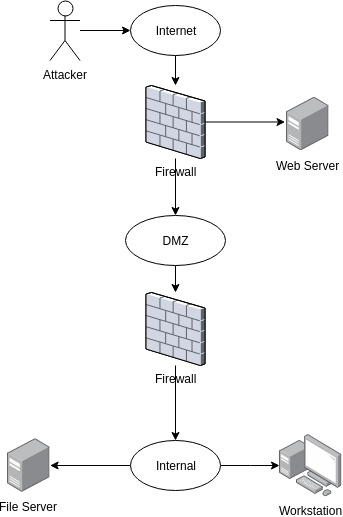
\includegraphics[trim=0cm 0cm 0cm 0cm, clip=true,width=.25\textwidth]{content/figs/egarch_01.png}
% \caption{Example network}
% \label{fig:eg_net01}
% \end{figure}

% \begin{figure}[ht]
% \centering
% \includegraphics[width=\linewidth]{content/figs/AttackGraph.eps}
% \caption{Resulting attack graph}
% \label{fig:eg_ag01}
% \end{figure} 

%  A brief reading of the attack graph generated in Table \ref{tab:eg_verts} and Figure \ref{fig:tg_001} from the top left:
% \setlist{nosep}
% \begin{itemize}
% \item An attacker from the internet (node 18) can access $webServer$ on port 80 (node 15)
% \item Vulnerability CAN-2002-0392 can be exploited (node 20) to allow remote code execution on $webServer$ as user $apache$. From here the attacker can either (node 13):
% \begin{enumerate}
% \item Access $fileServer$ directly over rpc (node 10) and use this to escalate privilege to root (node 22) and write malicious files served to $workstation$ (node 5). 
% \item $OR$ the attacker can write malicious files served to $workstation$ directly using NFS shell (node 23) 
% \end{enumerate}
% \item Given $workstation$ can access the malicious file (node 26) and the malicious file has been created (node 5) then $workstation$ can execute the malicious file with $root$ privileges allowing the attacker to achieve the target. 
% \end{itemize}


% \begin{table}[ht]
% \caption{VERTICES.csv}
% % \begin{subtable}[t]{0.45\textwidth}
% \resizebox{.48\textwidth}{!}{%
% % \begin{tabular}[t]{@{}llll@{}}
% \begin{tabular}[t]{@{}p{0.01\textwidth}p{0.25\textwidth}p{0.05\textwidth}p{0.05\textwidth}@{}}
% \toprule
% ID & Text & Type & Leaf \\ \midrule
% 1 & execCode(workStation, root) & OR & 0 \\ 
% 2 & RULE 4 (Trojan horse installation) & AND & 0 \\
% 3 & accessFile(workStation,write, '/usr/local/share') & OR & 0 \\
% 4 & RULE 16 (NFS semantics) & AND & 0 \\
% 5 & accessFile(fileServer ,write, '/export') & OR & 0 \\
% 6 & RULE 10 (execCode implies file access) & AND & 0 \\
% 7 & canAccessFile(fileServer, root, write, '/export') & LEAF & 1 \\
% 8 & execCode(fileServer, root) & OR & 0 \\
% 9 & RULE 2 (remote exploit of a server program) & AND & 0 \\
% 10 & netAccess(fileServer, rpc, 100005) & OR & 0 \\
% 11 & RULE 5 (multi-hop access) & AND & 0 \\
% 12 & hacl(webServer, fileServer, rpc, 100005) & LEAF & 1 \\
% 13 & execCode(webServer, apache) & OR & 0 \\
% 14 & RULE 2 (remote exploit of a server program) & AND & 0 \\
% 15 & netAccess(webServer, tcp, 80) & OR & 0 \\
% 16 & RULE 6 (direct network access) & AND & 0 \\
% 17 & hacl(internet,webServer, tcp, 80) & LEAF & 1 \\
% 18 & attackerLocated(internet) & LEAF & 1 \\
% 19 & networkServiceInfo(webServer, httpd, tcp, 80, apache) & LEAF & 1 \\
% 20 & vulExists(webServer, 'CAN-2002-0392',httpd, remoteExploit, privEscalation) & LEAF & 1 \\
% 21 & networkServiceInfo(fileServer, mountd, rpc, 100005, root) & LEAF & 1 \\
% 22 & vulExists(fileServer,vulID, mountd, remoteExploit, privEscalation) & LEAF & 1 \\
% 23 & RULE 17 (NFS shell) & AND & 0 \\
% 24 & hacl(webServer,fileServer, nfsProtocol, nfsPort) & LEAF & 1 \\
% 25 & nfsExportInfo(fileServer, '/export', write, webServer) & LEAF & 1 \\
% 26 & nfsMounted(workStation, '/usr/local/share', fileServer, '/export', read) & LEAF & 1 \\ \bottomrule
% \end{tabular}%
% }
% % \caption{VERTICES.csv}
% \label{tab:eg_verts}
% % \end{subtable}
% \end{table}

% % \begin{subtable}[t]{0.3\textwidth}
% \flushright
% \resizebox{.68\textwidth}{!}{%


% \begin{table}[ht]
% \caption{ARCS.CSV}
% % \resizebox{.48\textwidth}{!}{%
% \begin{tabular}[t]{@{}lll@{}}
% \toprule
% src vertex & dst vertex & weight \\ \midrule 
% 6  & 7  & -1 \\
% 11 & 12 & -1 \\
% 16 & 17 & -1 \\
% 16 & 18 & -1 \\
% 15 & 16 & -1 \\
% 14 & 15 & -1 \\
% 14 & 19 & -1 \\
% 14 & 20 & -1 \\
% 13 & 14 & -1 \\
% 11 & 13 & -1 \\
% 10 & 11 & -1 \\
% 9  & 10 & -1 \\
% 9  & 21 & -1 \\
% 9  & 22 & -1 \\
% 8  & 9  & -1 \\
% 6  & 8  & -1 \\
% 5  & 6  & -1 \\
% 23 & 24 & -1 \\
% 23 & 25 & -1 \\
% 23 & 13 & -1 \\
% 5  & 23 & -1 \\
% 4  & 5  & -1 \\
% 4  & 26 & -1 \\
% 3  & 4  & -1 \\
% 2  & 3  & -1 \\
% 1  & 2  & -1 \\ \bottomrule
% \end{tabular}
% % }

% \label{tab:eg_arcs}
% % \end{subtable}
%     % \label{tab:mulval_out}
% \end{table}

% Along with the visualization in Figure \ref{fig:tg_001}, MulVal also produces comma separated value formatted output which lends itself more readily to further analysis. The lists of edges and vertices in Tables \ref{tab:eg_verts} and \ref{tab:eg_arcs} describe the attack graph generated from Listing \ref{lst:input}.